\documentclass[12]{article}
\usepackage[spanish,english]{babel}
%\usepackage[spanish]{babel}
\usepackage[utf8]{inputenc}
\usepackage{graphicx}
\usepackage{epsfig}
\usepackage{multirow}
\usepackage{multicol,caption}
\usepackage{amsthm} % Theorem Formatting
\usepackage{amssymb}    % Math symbols such as \mathbb
\usepackage{color}
\usepackage{hyperref}
\usepackage[none]{hyphenat}
\usepackage{appendix}
\renewcommand{\appendixname}{Anexo}
\renewcommand{\appendixtocname}{LISTA DE ANEXOS}
\renewcommand{\appendixpagename}{Anexos}
%\renewcommand{\tablename}{Tabla}
%\def\tablename{Cuadro}% por \def\tablename{Tabla}% 
\newenvironment{Figure}
{\par\medskip\noindent\minipage{\linewidth}}
{\endminipage\par\medskip}
\addto\captionsspanish{%
\def\tablename{Tabla}%
}
\topmargin  = 10pt
\oddsidemargin  = -0.5in
%\headheight = 12pt
%\headsep    = 15pt
%\footskip   = 15pt
\textheight = 21.5 cm
\textwidth  = 18.5cm
\tolerance=10000
\title{\bf{Calculo de la longitud de onda de la radiación de un diodo led infrarrojo, utilizando el modulo motorizado infrarossi y su software de control Free infrarossi}}
\author{Julian Salamanca\footnote{jasalamanca@udistrital.edu.co}, Diego Parra\footnote{diegoestudianteud1@gmail.com} \\
  Universidad Distrital, Calle 3 No 26A-40 Bogotá-Colombia\\
  Grupo de Física e Informática ``FISINFOR''
}
\date{\today}
\begin{document}
%\def\tablename{Cuadro}% por \def \tablename{Tabla}% 
\renewcommand{\tablename}{Tabla}
\maketitle
\vspace{-0.8cm}
\selectlanguage{english}

\begin{abstract}
In this paper calculated the wavelength emitted by  an infrared LED diode using a diffraction grating, infrarossi motorized module and control software  free infrarossi; a GNU-Linux environment, highlighting the functionality of this instrument in illustrating the diffraction property of electromagnetic waves and the duality wave - corpuscle. \\
{\bf{Keywords:}} Motor module, infrared sensors, microcontroller module bluetooth, electromagnetic wave, diffraction.


\selectlanguage{spanish}
\begin{center}
{\bf{Resumen}} 
\end{center}
El presente trabajo calcula la longitud de onda emitida por un diodo led infrarrojo, utilizando una rejilla de difracción, el modulo motorizado  infrarossi y su software de control free infrarossi; en un entorno GNU-linux, resaltando la funcionalidad de este instrumento en la ilustración de la difracción como propiedad de la ondas electromagnéticas y su dualidad onda – corpúsculo. \\
{\bf{Descriptores:}} Modulo motorizado, sensores infrarrojos, microcontrolador, modulo bluetooth, ondas electromagnéticas, difracción. 
\end{abstract}

%tabla de contenido sin numeracion
%\renewcommand\contentsname{\centering TABLA DE CONTENIDO}
%\thispagestyle{empty}
%\setcounter{page}{1}
%\tableofcontents
%\clearpage

%lista de figuras
%\renewcommand\listfigurename{\centering LISTA DE FIGURAS}
%\listoffigures
%\clearpage

%lista de tablas
% \renewcommand\listtablename{\centering LISTA DE TABLAS}
% \listoftables
% \clearpage

\begin{multicols}{2}
\section{Introducción}
Los fenómenos de las ondas siempre han fascinado nuestros pensamientos y tratamos de acercarnos a estos fenómenos para tratar de entenderlos, es allí donde la física con ayuda de la matemática muestran su majestuosidad, al explicar de manera muy detallada estos fenómenos de transporte; la difracción es una de estas propiedades, la cual esta muy presente en la vida diaria y con la ayuda del modulo motorizado infrarossi y su software de control free infrarossi, se ilustra este fenómeno físico y se calcula la longitud de onda propia producida por un diodo infrarrojo. \\ \\``Un cuerpo opaco colocado a medio camino entre una pantalla y una fuente puntual proyecta una sombra complicada hecha en regiones claras y oscuras muy diferentes de las que podría esperarse de los principios básicos de la óptica geométrica. El trabajo de Franceso Grimaldi en el siglo XVII fue el primer estudio detallado que se publicó sobre esta desviación de la luz de su propagación rectilínea. A la que denomino difracción. El efecto es una característica general de los fenómenos ondulatorios que ocurren donde quiera que una parte de un frente de onda ya sea sonido, onda material o luz, esté obstruida de alguna manera. Si al encontrar un obstáculo transparente u opaco se altera la amplitud o la fase de una región del frente de onda, esto produciría difracción. Los varios segmentos del frente de onda que se propagan más allá del obstáculo interfieren, produciendo aquella distribución de densidad de energía particular denominada figura de difracción. No hay distinción física significativa entre interferencia y difracción. Sin embargo, se ha vuelto algo común, aunque no siempre apropiado, hablar de interferencia cuando se analiza la superposición de solamente unas pocas ondas y de difracción cuando se trata de un gran número de ondas. \\ \\
La red de difracción es un conjunto repetitivo de elementos difractores de una onda emergente, bien sean aberturas u obstáculos, que tienen el efecto de producir alteraciones periódicas en la fase, amplitud o ambas. Uno de los más simples de tales conjuntos es la configuración de rendijas múltiples. Parece que fue inventado por el astrónomo americano David Rittenhouse hacia 1785. Algunos años más tarde Joseph Von Fraunhofer redescubrió, por su cuenta, este principio y siguió aportando un buen número de contribuciones importantes tanto a la teoría como a la tecnología de redes.\\ \\ 
Los primeros dispositivos eran en realidad conjuntos de rendijas múltiples, que consistían por lo general en un retículo de alambre muy fino o hilo enrollado y extendido entre dos tornillos paralelos que servían como espaciadores. Al pasar a través de semejante sistema, un frente de onda se encuentra con regiones opacas y transparentes alternadas, sufriendo una modulación en amplitud. Así mismo, una configuración múltiple de rendijas se denomina red de transmisión de amplitud. Otra forma más corriente de red de transmisión se hace rayando o raspando  unas hendiduras paralelas en la superficie de una lámina de cristal clara y plana. Cada raspadura sirve como fuente de luz esparcida, formando juntas un conjunto regular de fuentes lineales paralelas. Cuando la red es totalmente transparente, de tal manera que la modulación en amplitud sea despreciable, las variaciones regulares del espesor óptico a través del retículo dan una modulación en fase y tenemos lo que se denomina red de transmisión de fase. En la representación de Huygens -Fresnel podemos visualizar los trenes de onda como radiados con diferentes fases sobre la superficie de la red. Un frente de onda emergente contiene, por consiguiente, unas variaciones periódicas en su forma más que en su amplitud lo cual, a su vez, equivale a una distribución angular de las ondas constitutivas. "\cite{OPTICA}
\selectlanguage{spanish}
\section{Marco teórico}
Los fotones producidos por el diodo emisor de la fuente emisora de radiación infrarroja antes de pasar estos por la rejilla de difracción se dan debido a que “en los semiconductores, con estructura compleja de las bandas energéticas, son posibles las transiciones indirectas de los electrones de la banda de conducción  a la de valencia acompañadas de la emisión de un fotón. En este caso la recombinación del electrón libre con el hueco se desarrolla con la aparición de un fonón, lo que asegura la conservación del cuasi impulso. Lo más probable es que el fonón sea emitido. Si en el semiconductor se desarrollan procesos de recombinación entre bandas  tanto directa como indirectas, en el espectro de radiación se observan dos bandas de luminiscencia. \\ \\
En la banda prohibida de los semiconductores reales existe una gran cantidad de estados localizados, que están ligados a los átomos de impureza, defectos de la estructura, infracciones de la periodicidad de la estructura en la superficie, etc. Estos estados localizados desempeñan un papel importante  en los procesos de luminiscencia. 
\begin{Figure}	
\center
\begin{tabular}{|l|r|}
\hline
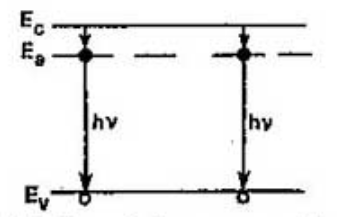
\includegraphics[width=6cm, height=6cm]{img/transiciones.png} \\ \hline
\end{tabular}
\captionof{figure}{Transiciones con radiación entre una banda y los estados de impureza.}
\label{fig:g1}
\end{Figure}
Las transiciones de los electrones de la banda de conducción a los niveles de los pequeños donadores (o de los huecos de la banda de valencia a los niveles de los pequeños aceptores),  que hacen que estos últimos se neutralicen, pueden ser con radiación.. En este caso es de esperar la aparición de luminosidad en la región infrarroja remota del espectro. Pero los cálculos  muestran que en estas transiciones lo más probable es que sea emitido un fonón y no un fotón, es decir, que el proceso se desarrolla sin radiación. La recombinación con radiación se produce por lo general  como viene mostrado en la figura 1. Primero un electrón de la banda de conducción es capturado por un nivel local situado un poco más abajo que Ec  \footnote{Ec es el nivel de energía de conducción.}, y después se efectúa la recombinación de este electrón localizado con un hueco de la banda de valencia, la cual va acompañada de la emisión de un fotón. El electrón puede también realizar una transición con radiación de la banda de conducción y después recombinarse con un hueco. \\ 
El estudio de los espectros de luminiscencia relacionados a diversas impurezas y defectos permite obtener información sobre estas infracciones de la estructura. \\ \\
Durante la absorción de la luz puede surgir en los semiconductores pares electrón – hueco ligados por la atracción coulombiana, es decir, excitones. Si uno de estos pares se aniquila, se produce la emisión de un fotón. La energía de esta radiación es: 
\begin{equation}
h\nu = E_g - E,
\end{equation}
donde E es la energía de enlace del excitón. \\ \\
Como el excitón puede tener estados excitados, la radiación dada a la recombinación excitónica puede consistir en una serie de rayas estrechas correspondientes a las transiciones desde los estados excitados." \cite{SEMICONDUCTOR} \\ \\
Una vez producido los fotones infrarrojos con energía $h\nu$ se hacen pasar por una red de difracción de 100 lineas por milímetro, a lo que esta radiación en vez de comportarse como un corpúsculo como lo venia haciendo, se comporta como una onda.
\\ \\
``Al reflejarse en esta clase de red, la luz esparcida por las varias caracteristicas periodicas de la superficie llegaran a un punto P con una relación de fase definida. El patrón de interferencia correspondiente engendrado despues de la reflexión es muy similar al que se produce por transmisión. Las redes diseñadas especificamente para funcionar de esta manera se denomina redes de reflexión de fase. Tradicionalmente, las redes de esta clase son rayadas sobre películas finas de aluminio que han sido evaporadas sobre bloques de vidrio ópticamente planos. Puesto que el aluminio es bastante blando, hay menos desgaste de la herramienta de rayar de diamante, siendo tambien mejor reflector en la región ultravioleta. \\ \\
Si miramos perpendicularmente a través de una red de transmisión hacia una fuente lineal paralela distante, los ojos servirían como lente de enfoque para la distribución de difracción. \\ \\ 
Como un puente simple aunque lógico entre los estudios de la interferencia y de la difracción se considera un conjunto de N osciladores puntuales coherentes (o antenas emisoras), todos ellos idénticos incluso en su polarización. Por ahora, hay que suponer que los osciladores no tengan diferencia de fase intrínseca, \footnote{Este es el caso ideal, el cual en el experimento se da el caso que los fotones infrarrojos producidos por el diodo led infrarrojo no están en fase} es decir, cada uno tiene el mismo ángulo de fase inicial. Todos los rayos son casi paralelos, encontrándose en un punto P muy distante. Si la extensión espacial del conjunto es comparativamente pequeña, las amplitudes de onda individuales que lleguen a P serán esencialmente iguales , habiendo recorrido casi las mismas distancias, esto es:
\begin{equation}
E_{0}(r_{1}) = E_{0}(r_{2})= ... = E_{0}(r_{n}) = E_{0}(r)
\end{equation}
La suma de los trenes de onda esféricos interferentes   produce un campo eléctrico  en P proporcionado por la parte real de 
\begin{equation}
\vec{E} = E_{0}(r)e^{i(kr_{1} - \omega t)} +  E_{0}(r)e^{i(kr_{2} - \omega t)} + ... +  E_{0}(r)e^{i(kr_{N} - \omega t)}
\end{equation}
Por tanto ahora 
\begin{equation}
\vec{E} = E_{0}(r)e^{(-i\omega t)}e^{ikr_{1}}\times[1 + e^{ik(r_{2}-r_{1})} + e^{ik(r_{3}-r_{1})} + ... + e^{ik(r_{N}-r_{1})}]
\end{equation}
La diferencia de fases entre fuentes adyacentes se obtiene de la expresión $\delta = k_{0}\Lambda$, y puesto que $\Lambda = ndsin(\theta)$, en un medio con índice n, $\delta  = kdsin(\theta)$, de esto se deduce que $\delta = k(r_{2}-r_{1}) $, $2\delta = k(r_{3}-r_{1}) $, etc. Entonces el campo de P puede escribirse como:
\begin{equation}
\vec{E} = E_{0}(r)e^{(-i\omega t)}e^{ikr_{1}} \times[1 + (e^{i\delta}) +  (e^{i\delta})^{2} + (e^{i\delta})^{3} + ... + (e^{i\delta})^{N-1}]
\end{equation}
La serie geométrica entre paréntesis tiene el valor: 
\begin{center}
$(e^{i\delta N} -1)/(e^{i\delta} -1) $
\end{center}
que puede ordenarse así:
\begin{equation}
\frac{e^{i\delta N/2}[e^{i\delta N/2} - e^{-i\delta N/2}]} {e^{i\delta /2}[e^{i\delta /2} - e^{-i\delta /2}]}
\end{equation}
o de manera equivalente
\begin{equation}
e^{i(N -1)\delta/2} * \left( \frac{sin(N\delta /2)}{sin(\delta /2)} \right )
\end{equation}
Entonces el campo se transforma en:
\begin{equation}
\vec{E} = E_{0}(r)e^{(-i\omega t)}e^{i[kr_{1} + (N -1)\delta/2]}* \left ( \frac{sin(N\delta /2)}{sin(\delta /2)} \right )
\end{equation}
Si se define R como  como la distancia desde el centro de la linea de los osciladores hasta el punto P, es decir:
\begin{equation}
R = \frac{1}{2}(N-1)d sin(\theta) + r_{1}
\end{equation}
Entonces la ecuación 8 se convierte en:
\begin{equation}
\vec{E} = E_{0}(r)e^{i(kR - \omega t)} \left ( \frac{sin(N\delta /2)}{sin(\delta /2)} \right )
\end{equation}
Finalmente, la distribución de densidad de flujo dentro de la distribución de difracción debida a N fuentes puntuales distantes, idénticas y coherentes en una disposición lineal, es proporcional a $EE^{*}/2$ para $E$ compleja  o
\begin{equation}
I = I_{0}\frac{sin^{2}(N\delta/2)}{sin^{2}(\delta/2)}
\end{equation}
donde $I_{0}$ es la densidad de flujo que saliendo desde cualquier fuente puntual llegue a P. La dependencia funcional de $I$ con $\theta$ queda más clara en la forma 
\begin{equation}
I = I_{0}\frac{sin^{2}[(Nk\delta/2)sin(\theta)]}{sin^{2}[(k\delta/2)sin(\theta)]}
\end{equation}
\\ \\
El término $sin^{2}[(Nk\delta/2)sin(\theta)]$ se somete a unas fluctuaciones rápidas, mientras que las fluctuación que la modula, $sin^{-2}[(k\delta/2)sin(\theta)]$, varia de manera relativamente lenta. La expresión combinada da lugar a una serie de picos principales agudos separados por picos pequeños complementarios.\\ \\
La ecuación que describe el fenomeno físico se denomina ecuación de red para incidencia normal. 
\begin{equation}
d*sin(\theta _m)= m\lambda 
\end{equation}
Los valores de de m especifican el orden de diversos máximos principales. Para una fuente que tenga un espectro continuo ancho, la imagen de orden cero, $ m = 0 $, corresponde a la imagen blanca de la fuente no desviada $ \theta _0 = 0 $. La ecuación de red depende de $\lambda$ y así, para cualquier valor de m $\ne  0$, las distintas imágenes coloreadas de la fuente correspondientes a ángulos ligeramente diferentes $(\theta _m)$, se dispersa en un espectro continuo. Las regiones ocupadas por los débiles máximos secundarios aparecerán como bandas aparentemente desprovistas de luz. El espectro de primer orden $m = \frac{+}{-}1$ aparece a cada lado de $\theta = 0$ y es seguido, junto con intervalos alternados de oscuridad, por los espectros de orden superior, $m = \frac{+}{-}1, \frac{+}{-}2$, etc. "\cite{OPTICA} \\ \\
Ahora se produce un patrón de difracción que alcanza al detector infrarrojo del modulo motorizado Free infrarossi, el cual avanza en linea recta a 45 centímetros de la fuente emisora de fotones infrarrojos, perpendicular a la incidencia de los patrones de difracción. \\\\
El detector del modulo motorizado Free infrarossi es un diodo receptor infrarrojo; “cuando un haz de radiación monocromática u homogénea traspasa una sustancia, debido a la reflexión y absorción su intensidad disminuye. Supongamos que la fracción de energía reflejada en el extremo del cuerpo sea $R$ , magnitud  que lleva el nombre de factor de reflexión. Si la intensidad de la luz incidente es $I_{0}$ y la reflejada $I_{R}$, entonces 
\begin{equation}
R = \frac{I_{R}}{I_{0}}
\end{equation}
La dependencia del factor de reflexión respecto a la frecuencia $R(\omega)$ o de la longitud de onda $R(\lambda)$ se llama espectro de reflexión.
Designemos por $I$ la intensidad de la luz que incide en la capa $dx$, cómo se muestra en la figura 2. En tal caso, debido a la absorción de la luz en esta capa la intensidad de radiación se reduce en la magnitud $dI$ La cantidad de energía absorbida $dI$ es proporcional a la cantidad de energía incidente   en la capa y el espesor de la capa absorbente:
\begin{equation}
-dI = \alpha I dx
\end{equation}
El coeficiente de proporcionalidad $\alpha$, que expresa la cantidad de energía absorbida del haz de intensidad unidad por la capa de espesor unidad, se llama factor de absorción.
\begin{Figure}	
\center
\begin{tabular}{|l|r|}
\hline
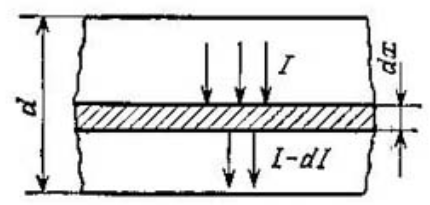
\includegraphics[width=5cm, height=5cm]{img/absorcionsemiconductor.png} \\ \hline
\end{tabular}
\captionof{figure}{Absorción de la luz por un semiconductor.}
\label{fig:g2}
\end{Figure}
Integrando la ecuación 15 sin tener en cuenta la reflexión 
\begin{equation}
\int_{Io}^{I} \frac{dI}{I} = - \int_{0}^{d} \alpha dx 
\end{equation}
se obtiene la expresión 
\begin{equation}
I = I_{0}e^{- \alpha d}
\end{equation}
conocida con el nombre de ley de Buger – Lambert. La magnitud $\alpha$ es una caracteristica del medio absorbente y depende la longitud de onda de la radiación. La dependencia del factor de absorción respecto de la frecuencia $\alpha(\omega)$ o de la longitud de onda $\alpha(\lambda)$ se llama espectro de absorción de la sustancia.
\\ \\
Suponiendo que se tiene $N$ centros de absorción. Designamos por $\sigma$ la probabilidad de absorción de un haz monofotón por un centro de absorción de un fotón en la unidad de tiempo. La sección eficaz $\sigma$ depende de la energía del fotón y de la naturaleza de los centros absorbentes.
De acuerdo con la ecuación $(\sigma N)^{-1}$ que es la longitud media de recorrido libre de un fotón $l_{f}$ en un medio absorbente, es decir,
\begin{equation}
l_{f} = \frac{1}{\sigma N}
\end{equation}
Mientras que el factor de absorción 
\begin{equation}
\alpha = \frac{1}{l_{f}}
\end{equation}
es la probabilidad de absorción de un fotón en la unidad de longitud. Suponiendo que en el semiconductor existen centros de absorción de diferente naturaleza. Si $N_{l}$ centros de absorción se caraccterizan por la sección eficaz $\sigma_{i}$, entonces
\begin{equation}
\alpha_{i}(\omega) = \sigma_{i} N_{l}
\end{equation}
el factor de absorción total de la sutancia $\alpha$ es la suma de los factores de absorción parciales:
\begin{equation}
\alpha(\omega) = \sum_{i} \alpha_{i}(\omega) = \sum_{i} \sigma_{i}(\omega)N_{l}
\end{equation}
Por lo tanto, el espectro de absorción total se compone de los espectros de absorción de los distintos centros de absorción. \\\\
Al interactuar los electrones del semiconductor con la radiación electromagnética deben cumplirse dos leyes: la ley de conservación de la energía  $E$ y la ley de conservación del casi impulso $\textbf{p}$, y después de interactuar se tiene $E'$ y $\textbf{p'}$, estas leyes se escriben en la forma 
\begin{equation}
E' = E + \hbar \omega
\end{equation}
\begin{equation}
\textbf{p'} = \textbf{p} + \hbar \bar{\eta}
\end{equation}
La absorción de la radiación en los semiconductores puede estar vinculada con la variación del estado energético de los electrones libres o enlazados con los átomos, así como la variación de la energía vibratoria (oscilante)de los átomos de la red. Debido a esto, en los semiconductores se distinguen cinco tipos fundamentales  de absorción óptica: intrínseca, excitónica, por portadores de carga libres, extrínseca y absorción de la luz por la red cristalina."\cite{ESTADO_SOLIDO} \\\\
Una vez absorbidos los fotones infrarrojos, el microcontrolador atmega 328 del vehículo motorizado free infrarossi, mide la energía utilizada en el proceso de movilidad de las partículas cargadas en el diodo y esta información es enviada vía bluetooth al ordenador.
%----------------------aca empieza el montaje experimental-------------------------
\section{Montaje experimental}
\subsection{Materiales del montaje}
Para la realización de este montaje se utilizarón los siguientes materiales:
\begin{enumerate}
\item[a.] Ordenador con sistema operativo GNU-Linux.
\item[b.] Modulo motorizado infrarossi.
\item[c.] Software de control free infrarossi.
\item[d.] Fuente emisora de fotones infrarrojos.
\item[e.] Modulo bluetooth para pc.
\item[f.] Rejilla de difracción de 100 lineas por milímetro 
\end{enumerate}
%--------------------Montaje-------------------------------------------------
\subsection{Montaje}
Colocar la fuente\footnote{Esta fuente se elaboro con un diodo led infrarrojo de 800 nm y un encapsulado epoxi de 3 mm.} emisora de fotones infrarrojos con la red de difración de 100 lineas por milímetro, frente a ella colocar el modulo motorizado infrarossi a 45 cm de la fuente emisora, como se muestra en la figura 3. 
\begin{Figure}	
\center
\begin{tabular}{|l|r|}
\hline
\\
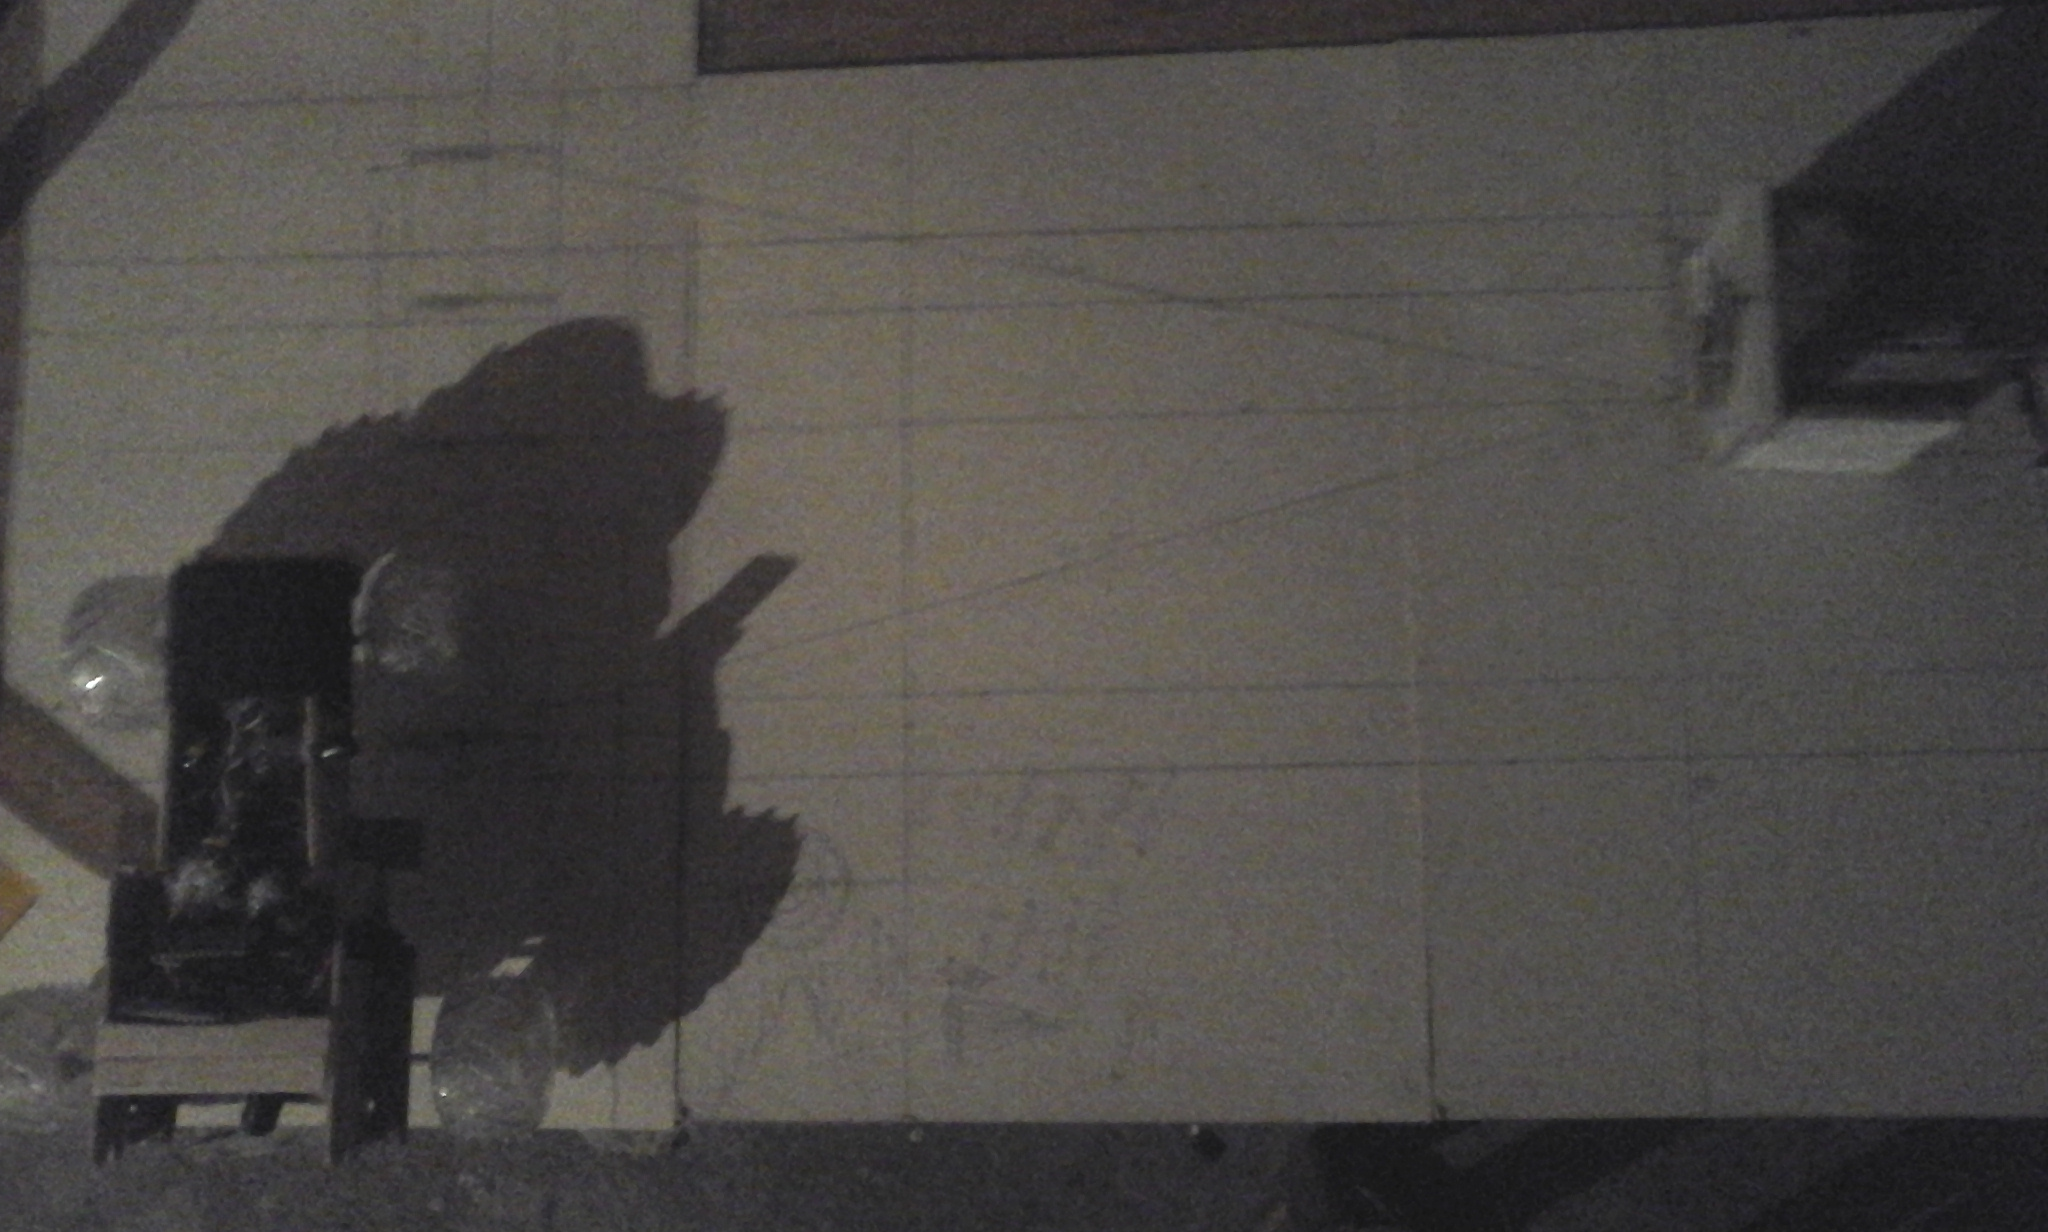
\includegraphics[width=9cm, height=7cm]{img/mon_difraccion.png} \\\\ \hline
\end{tabular}
\captionof{figure}{Imagen del montaje para la difracción utilizando el modulo motorizado infrarossi, una fuente emisora de fotones de $\lambda = 800 nm$  y una red de difracción de 100 lineas por milímetro.}
\label{fig:g3}
\end{Figure}
\vspace{1cm}
Abrir una terminal de GNU-Linux y escribir infrarossi, oprimir enter y la clave de superusuario, luego de abrir el programa debe oprimir el boton on, esperar que se empareje el bluetooth, una vez emparejado el bluetooth el programa desplegara un tercer menú, oprimir el botón de difracción y esperar que el programa tome los datos necesarios.\\ \\
Luego de capturar los datos aparecerá la gráfica de los datos, oprima doble click izquierdo en el máximo de interferencia y sin soltar el cursor lleve la linea al siguiente máximo de interferencia,  suelte el botón del cursor e inmediatamente  aparecerá la gráfica con el análisis de longitud de onda infrarroja del diodo, tal como se muestra en la figura 4. \\\\
La gráfica de análisis y los datos capturados se almacenan dentro del archivo llamado Carpetas/Difraccion con la fecha y hora del análisis de datos.
\begin{Figure}	
\center
\begin{tabular}{|l|r|}
\hline
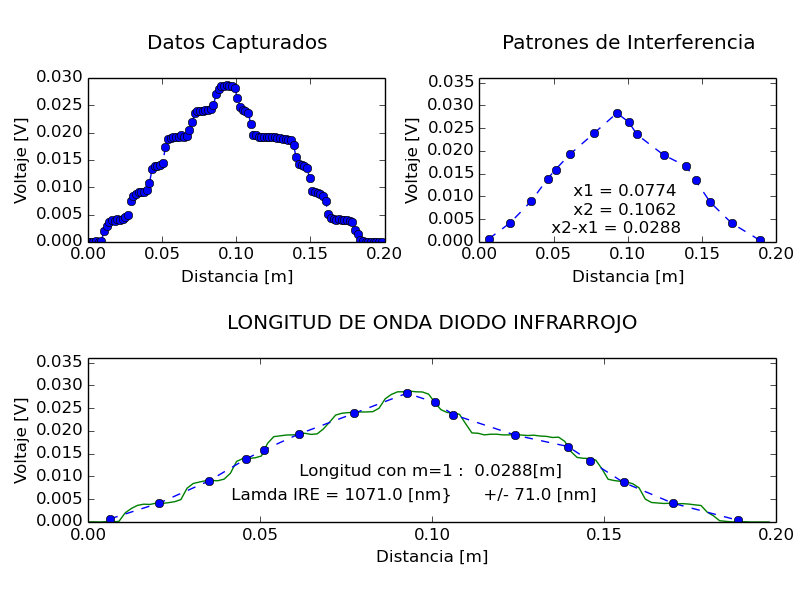
\includegraphics[width=8cm, height=6cm]{img/Graficas.png} \\ \hline
\end{tabular}
\captionof{figure}{Imagen generada por el programa free infrarossi.}
\label{fig:g4}
\end{Figure}
\section{Análisis de resultados}
El programa free infrarossi cuando termina de recoger los datos realiza un análisis estadístico de los mismos, en una ventana aparte realiza la gráfica de los datos y predice la longitud de onda del diodo emisor infrarrojo con un error en la medida aceptable, no superior al $15\%$ dependiendo de la rigurosidad en el montaje.\\\\
En la tabla 1, se muestra los resultados de nueve experimentos para calcular la longitud de onda $\lambda$ de la radiación producida por un diodo led emisor infrarrojo, fueron capturados y analizados con el modulo motorizado infrarossi y su software de control free infrarossi. $\Delta X$ es la distancia que hay entre pico y pico del patrón obtenido, esta viene en metros; $\lambda$ exp.  es la longitud de onda obtenida a través del experimento, viene en nanometros; $\lambda$ teo. Es la longitud de onda teórica del diodo emisor infrarrojo,  la cual corresponde a $800 nm$; el error porcentual es la ultima columna  de la tabla.

\begin{center}
\begin{tabular}{|c|c|c|c|c|} 
\hline
\bf{Prueba} & \textbf{$\Delta$X [m]} & \bf{$\lambda$exp.[nm]} & \bf{$\lambda$teo.[nm]} & \bf{error  \%} \\
\hline
 1 & 0.0393 & 836 & 800 & 4.62\\
\hline
 2 & 0.0385 & 820 & 800 & 2.506\\
\hline
 3 & 0.0393 & 836 & 800 & 4.62\\
\hline 
 4 & 0.0341 & 727 & 800 & 9.138\\
\hline
5 & 0.0345 & 735 & 800 & 8.978\\
\hline
6 & 0.0341 & 727 & 800 & 9.138\\
\hline
7 & 0.0337 & 718 & 800 & 10.198\\
\hline
8 & 0.0333 & 709 & 800 & 11.257\\
\hline
9 & 0.0349 & 744 & 800 & 7.019\\
\hline
\end{tabular}
\\
\end{center}
\textbf{Tabla 1.} Datos obtenidos de nueve pruebas para medir la longitud de onda producida por un diodo emisor infrarrojo, con el modulo motorizado infrarossi y su software de control free infrarossi. 
\section{Conclusiones}
\begin{enumerate}
\item[*] La longitud de onda media del experimento es de $\bar{\lambda}_{exp} = 761 nm$, la cual difiere en $39 nm$ de la longitud de onda del diodo emisor infrarrojo.
\item[*] El modulo motorizado infrarossi y su software de control ilustran de manera cuantitativa y cualitativa fenómenos ondulatorios como la difracción e interferencia de las ondas electromagnéticas, calculando de manera aproximada su longitud de onda $\lambda$, con error inferior al $15\%$.   
\item[*] El modulo motorizado infrarossi y su software de control es una herramienta fácil de usar y muy precisa, capaz de ser utilizada para diversos propósitos en el aula de clase como modelo pedagógico,  tanto de profesionales como estudiantes de ciencias exactas.
\item[*] La física que se encuentra de manera implícita y explicita en este trabajo hace que el instrumento motorizado infrarossi y su software de control free infrarossi sea un herramienta indispensable  en el aula de clase.
\end{enumerate}
\vspace{1cm}
% ---------------------Aca empieza la bibliografia----------------------------------------------
\begin{thebibliography}{99}
\bibitem{OPTICA} Hecht, E., Dal Col, R., Talavera, R. W., \& Pérez, J. M. G. (2000). Óptica. Addison Wesley.
\bibitem{SEMICONDUCTOR} Shalímova, K. V., \& Grdiam, A. (1975). Física de los Semiconductores.
\bibitem{ESTADO_SOLIDO} Pavlov, P. V., \& Jojlov, A. F. (1987). Física del estado sólido. Rubiños-1860.
\bibitem{CIRCUITOS} Alexander, C. K., Sadiku, M. N., Bermúdez, A. V., \& Pedraza, C. R. C. (2006). Fundamentos de circuitos eléctricos. McGraw-Hill. 
\bibitem{PYTHON} Gift, N., \& Jones, J. M. (2008). Python for Unix and Linux system administration. ``O'Reilly Media, Inc.".
\bibitem{BASH} Álamos Zorrilla, J. (2004). Programación orientada a objetos con shell-bash. SÓLO PROGRAMADORES LINUX.
\end{thebibliography}
\end{multicols}
\end{document}
